\documentclass[11pt,a4paper]{article}

\usepackage[T1]{fontenc}
\usepackage[utf8]{inputenc}
\usepackage{lmodern}
\usepackage[margin=2.2cm]{geometry}
\usepackage{graphicx}
\usepackage{booktabs}
\usepackage{siunitx}
\usepackage{amsmath,amssymb}
\usepackage[version=4]{mhchem}
\usepackage{caption}
\usepackage{subcaption}
\usepackage{xcolor}
\usepackage{float}
\usepackage[hidelinks]{hyperref}

\sisetup{detect-all}
\setlength{\emergencystretch}{2em}
\captionsetup{font=small,labelfont=bf}
\graphicspath{{figures/}}

\title{CLYC Full-Energy Peak Efficiency versus Source Distance\\[2pt]
\large Simulation and Measurement Validation for the DCS-Monitor}
\author{DCS-Monitor simulation notes}
\date{\today}

\begin{document}

\maketitle

\begin{abstract}
The DCS-Monitor uses a CLYC scintillator to detect gamma radiation from a
spent-fuel cask. This report compares the simulated full-energy peak efficiency
of the CLYC detector with a nine-point measurement at source-to-detector
distances of \SI{200}{mm}, \SI{300}{mm}, and \SI{400}{mm} and gamma energies of
\SI{661.64}{keV}, \SI{1173.23}{keV}, and \SI{1332.51}{keV}. The simulation uses
\num{1e7} incident gammas per point, an isotropic point source at the centre of
a \SI{2}{mm}-thick epoxy source puck, and the full CLYC detector and casing
geometry. The measured efficiencies are taken from
\texttt{effDist\_clyc1.csv}; the column labelled \texttt{Efficiency (\%)} is a
factor \num{1000} larger than the value obtained from the measurement formula,
so the corrected measured efficiency is that column divided by \num{1000}.

At \SI{661.64}{keV}, the simulation and measurement agree within
\SI{9}{\percent}: the simulation-to-measurement ratios are
\num{1.059}, \num{0.963}, and \num{0.915} at \SI{200}{mm}, \SI{300}{mm}, and
\SI{400}{mm}. At \SI{1173.23}{keV}, the simulation is \num{1.48}--\num{1.70}
times the measurement, a discrepancy of \num{4}--\num{8} standard deviations
using the simulation statistical error. At \SI{1332.51}{keV}, the ratios are
\num{1.353}, \num{1.213}, and \num{1.014}; the first two points are
\num{4.7} and \num{2.2} standard deviations high, while the \SI{400}{mm} point
is consistent with the measurement but has an \SI{11.9}{\percent} statistical
uncertainty. The measured \SI{1173.23}{keV}/\SI{1332.51}{keV} ratio is
\num{0.94}, \num{0.92}, and \num{0.90}, whereas the reference column of the CSV
gives \num{1.21} and the simulation gives \num{1.18}, \num{1.12}, and
\num{1.49}. The measured ratio is therefore inverted relative to both the
reference and the simulation. A no-puck control at \SI{200}{mm} and
\SI{661.64}{keV} gives \num{0.00876(30)}\,\% versus \num{0.00843(29)}\,\% with
the puck, so the epoxy puck changes the efficiency by
\SI{3.8 \pm 4.8}{\percent}, consistent with zero. The \SI{661.64}{keV}
agreement validates the geometry, the source distance, and the analysis chain
at the \SI{10}{\percent} level. The energy-dependent discrepancy at
\SI{1173.23}{keV} and \SI{1332.51}{keV} is not explained by the source puck;
the most plausible remaining cause is that the simulation uses one
monoenergetic gamma per event and does not model the \SI{1173.23}--%
\SI{1332.51}{keV} cascade of \ce{^{60}Co} or the detector response. A cascade
source, a detector response model, and the measured spectra are the next
validation steps.
\end{abstract}

\tableofcontents

\section{Motivation and scope}

The DCS-Monitor simulation must predict the CLYC count rate for a source at a
known distance. A full-energy peak efficiency that is wrong by a factor of
\num{1.5} would change the inferred activity or the alarm threshold by the same
factor. The measurement in \texttt{effDist\_clyc1.csv} provides nine
independent points: three distances and three gamma lines. This report uses
those points to test the detector geometry, the source placement, and the
analysis chain.

The scope is deliberately narrow. The simulation is a Geant4 transport of
monoenergetic gammas through the CLYC detector and its casing. It does not
simulate scintillation light, light collection, or the electronics. The
efficiency is defined as the number of events whose total energy deposition in
the crystal lies within $\pm\SI{2}{\percent}$ of the incident gamma energy,
divided by the number of incident gammas. The measurement is the full-energy
peak efficiency obtained from the net peak area, the source activity, the
emission probability, and the measurement time. The two definitions are
compared at the same nominal source-to-detector distance.

The report is a validation note, not a final calibration. The statistical
uncertainties are reported; the systematic uncertainties of the source
activity, the distance, the detector geometry, and the peak fitting are not yet
included. The conclusions are therefore statements about the consistency of
the present simulation and data, not a complete uncertainty budget.

\section{Experimental data}

The measurement file is
\texttt{/home/turko46/data/CLYC\_validation/effDist\_clyc1.csv}. It contains
nine rows: \ce{^{137}Cs} at \SI{661.64}{keV} and \ce{^{60}Co} at
\SI{1173.23}{keV} and \SI{1332.51}{keV}, each at \SI{200}{mm},
\SI{300}{mm}, and \SI{400}{mm}. The detector is labelled CLYC1. The initial
activities are \SI{4.77e6}{Bq} for \ce{^{137}Cs} and \SI{18.50e6}{Bq} for
\ce{^{60}Co}; the current activities at the measurement dates are
\SI{3.65e6}{Bq} and \SI{11.31e6}{Bq}, respectively. The measurement time is
\SI{600}{s} for every row.

The experimental efficiency is
\begin{equation}
  \epsilon_{\mathrm{exp}}
  = \frac{N_{\mathrm{peak}}}{A(t)\,p_\gamma\,t}\times 100,
  \label{eq:eff-exp}
\end{equation}
where $N_{\mathrm{peak}}$ is the net peak area, $A(t)$ is the current activity
in becquerel, $p_\gamma=P_\gamma/100$ is the emission probability per decay,
and $t$ is the measurement time in seconds. For the \SI{200}{mm}
\SI{661.64}{keV} row,
\begin{equation}
  \epsilon_{\mathrm{exp}}
  = \frac{148423}{(3.65\times10^6)(0.8510)(600)}\times 100
  = \SI{0.00796}{\percent}.
  \label{eq:eff-exp-example}
\end{equation}
The CSV column labelled \texttt{Efficiency (\%)} contains \num{7.96} for this
row, which is exactly \num{1000} times the result of
Eq.~\eqref{eq:eff-exp-example}. The same factor of \num{1000} applies to all
nine rows. The corrected measured efficiency used in this report is therefore
\begin{equation}
  \epsilon_{\mathrm{meas}} = \frac{\texttt{Efficiency (\%)}}{1000}.
  \label{eq:csv-correction}
\end{equation}
The origin of the factor is not documented in the CSV. It is not caused by the
emission probability: using $P_\gamma$ as a percentage instead of a fraction
would change the result by a factor of \num{100}, not \num{1000}. The factor is
consistent across all rows, so it is treated as a column-normalisation error
and corrected once.

The CSV also contains an \texttt{Efficiency Reference Value (\%)} column with
values \num{6.64}, \num{3.14}, and \num{2.60} for the three energies. This
column is not the measured efficiency and is not used as the denominator in
this report. It is used only to compare the energy dependence: its
\SI{1173.23}{keV}/\SI{1332.51}{keV} ratio is \num{1.21}. The measured ratio is
\num{0.94}, \num{0.92}, and \num{0.90}; the simulation ratio is \num{1.18},
\num{1.12}, and \num{1.49}. The reference column therefore follows the
simulation better than the measurement, which is one of the central results of
this report.

\begin{table}[H]
  \centering
  \caption{Experimental data from \texttt{effDist\_clyc1.csv}. The column
  \texttt{eff}$_{\mathrm{CSV}}$ is the CSV value; the column
  \texttt{eff}$_{\mathrm{meas}}$ is that value divided by \num{1000}, following
  Eq.~\eqref{eq:csv-correction}. The current activity $A(t)$ is used in
  Eq.~\eqref{eq:eff-exp}.}
  \label{tab:data}
  \small
  \setlength{\tabcolsep}{4pt}
  \begin{tabular}{@{}rrrrrrrrr@{}}
    \toprule
    $d$ [mm] & Nuclide & $E$ [keV] & $A(t)$ [Bq] & $P_\gamma$ [\%] &
    $t$ [s] & $N_{\mathrm{peak}}$ & eff$_{\mathrm{CSV}}$ [\%] &
    eff$_{\mathrm{meas}}$ [\%] \\
    \midrule
    200 & \ce{^{137}Cs} & 661.64  & \num{3.65e6} & 85.10 & 600 & 148423 & 7.96 & 0.00796 \\
    200 & \ce{^{60}Co}  & 1173.23 & \num{11.31e6} & 99.97 & 600 & 153103 & 2.26 & 0.00226 \\
    200 & \ce{^{60}Co}  & 1332.51 & \num{11.31e6} & 99.99 & 600 & 163177 & 2.41 & 0.00241 \\
    300 & \ce{^{137}Cs} & 661.64  & \num{3.65e6} & 85.10 & 600 & 74617  & 4.00 & 0.00400 \\
    300 & \ce{^{60}Co}  & 1173.23 & \num{11.31e6} & 99.97 & 600 & 76163  & 1.12 & 0.00112 \\
    300 & \ce{^{60}Co}  & 1332.51 & \num{11.31e6} & 99.99 & 600 & 82693  & 1.22 & 0.00122 \\
    400 & \ce{^{137}Cs} & 661.64  & \num{3.65e6} & 85.10 & 600 & 41666  & 2.24 & 0.00224 \\
    400 & \ce{^{60}Co}  & 1173.23 & \num{11.31e6} & 99.97 & 600 & 42612  & 0.63 & 0.00063 \\
    400 & \ce{^{60}Co}  & 1332.51 & \num{11.31e6} & 99.99 & 600 & 47252  & 0.70 & 0.00070 \\
    \bottomrule
  \end{tabular}
\end{table}

\section{Geometry and source model}

\subsection{CLYC detector and source puck}

The detector is a CLYC scintillator with a \SI{25}{mm} diameter and a
\SI{25}{mm} length. The crystal front face is \SI{2}{mm} behind the detector
front plane. The crystal is mounted in the detector body and magnesium shield
described by \texttt{GeometryCLYC.cc}; the body is included in the simulation,
so the gamma must traverse the detector entrance window and the surrounding
material before reaching the crystal. The crystal density is
\SI{3.31}{g\,cm^{-3}}.

The source is an epoxy puck with a radius of \SI{10}{mm}, a thickness of
\SI{2}{mm}, and a density of \SI{1.16}{g\,cm^{-3}}. The gamma source is at the
puck centre. The puck is centred on the detector axis at
$(0,0,d)$, where $d$ is the nominal source-to-detector distance. Because the
crystal front face is \SI{2}{mm} behind the detector front plane, the
crystal-to-source distance is $d+\SI{2}{mm}$. The source is isotropic in the
production runs. The event-display macros described in
Section~\ref{sec:vis} use a focused source only to make the tracks visible;
they are not the production source model.

\subsection{Geometric acceptance}

For a point source on the detector axis and a circular crystal face of radius
$r$, the fraction of the full solid angle subtended by the face is
\begin{equation}
  \epsilon_\Omega(d)
  = \frac{1}{2}\left(1-\frac{d}{\sqrt{d^2+r^2}}\right),
  \label{eq:omega}
\end{equation}
where $d$ is the crystal-to-source distance and $r=\SI{12.5}{mm}$. Using
$d=d_{\mathrm{nom}}+\SI{2}{mm}$ gives
\begin{equation}
  \epsilon_\Omega =
  \begin{cases}
    \SI{0.0955}{\percent}, & d_{\mathrm{nom}}=\SI{200}{mm},\\
    \SI{0.0428}{\percent}, & d_{\mathrm{nom}}=\SI{300}{mm},\\
    \SI{0.0242}{\percent}, & d_{\mathrm{nom}}=\SI{400}{mm}.
  \end{cases}
  \label{eq:omega-values}
\end{equation}
The geometric acceptance is not the detection efficiency. It is the fraction
of emitted gammas that intersect the crystal front face. The intrinsic
efficiency is the ratio of the full-energy peak efficiency to
$\epsilon_\Omega$; it removes the leading $1/d^2$ dependence and is useful for
comparing the three distances.

\begin{table}[H]
  \centering
  \caption{Reference detector and source geometry. The crystal-to-source
  distance is the nominal distance plus \SI{2}{mm} because the crystal front
  face is recessed behind the detector front plane. The geometric acceptance
  follows Eq.~\eqref{eq:omega}.}
  \label{tab:geometry}
  \begin{tabular}{@{}lll@{}}
    \toprule
    Quantity & Value & Note \\
    \midrule
    Crystal material & CLYC & \SI{3.31}{g\,cm^{-3}} \\
    Crystal dimensions & \SI{25}{mm} $\times$ \SI{25}{mm} & diameter $\times$ length \\
    Crystal front face & \SI{2}{mm} behind detector front & recessed \\
    Detector body & \SI{29}{mm} snout & magnesium shield behind \\
    Source puck material & epoxy & \SI{1.16}{g\,cm^{-3}} \\
    Source puck dimensions & \SI{10}{mm} radius, \SI{2}{mm} thick & disc \\
    Source position & puck centre & $(0,0,d)$ \\
    Nominal distances & \SI{200}{mm}, \SI{300}{mm}, \SI{400}{mm} & source to detector front \\
    Crystal-to-source distance & $d+\SI{2}{mm}$ & used in Eq.~\eqref{eq:omega} \\
    Geometric acceptance & \num{0.0955}, \num{0.0428}, \num{0.0242}\,\% &
    at \SI{200}{mm}, \SI{300}{mm}, \SI{400}{mm} \\
    \bottomrule
  \end{tabular}
\end{table}

\subsection{Visual check of the detector and source}
\label{sec:vis}

Figure~\ref{fig:vis} shows two Geant4/OpenGL views of the detector, the source
puck, and ten \SI{661.64}{keV} gamma tracks. The source is at \SI{200}{mm}.
The top panel is a side view along the detector axis; the bottom panel is an
oblique view. The detector body is drawn semi-transparently so that the
crystal and the tracks inside the body are visible. The orange disc is the
source puck. The tracks are green; several leave the detector body, which is
expected for an isotropic source and a finite crystal. The source in these
renders is focused toward the detector to keep the ten tracks in the field of
view; the production runs use an isotropic source, so the renders are
illustrative and are not used to compute the efficiency.

\begin{figure}[H]
  \centering
  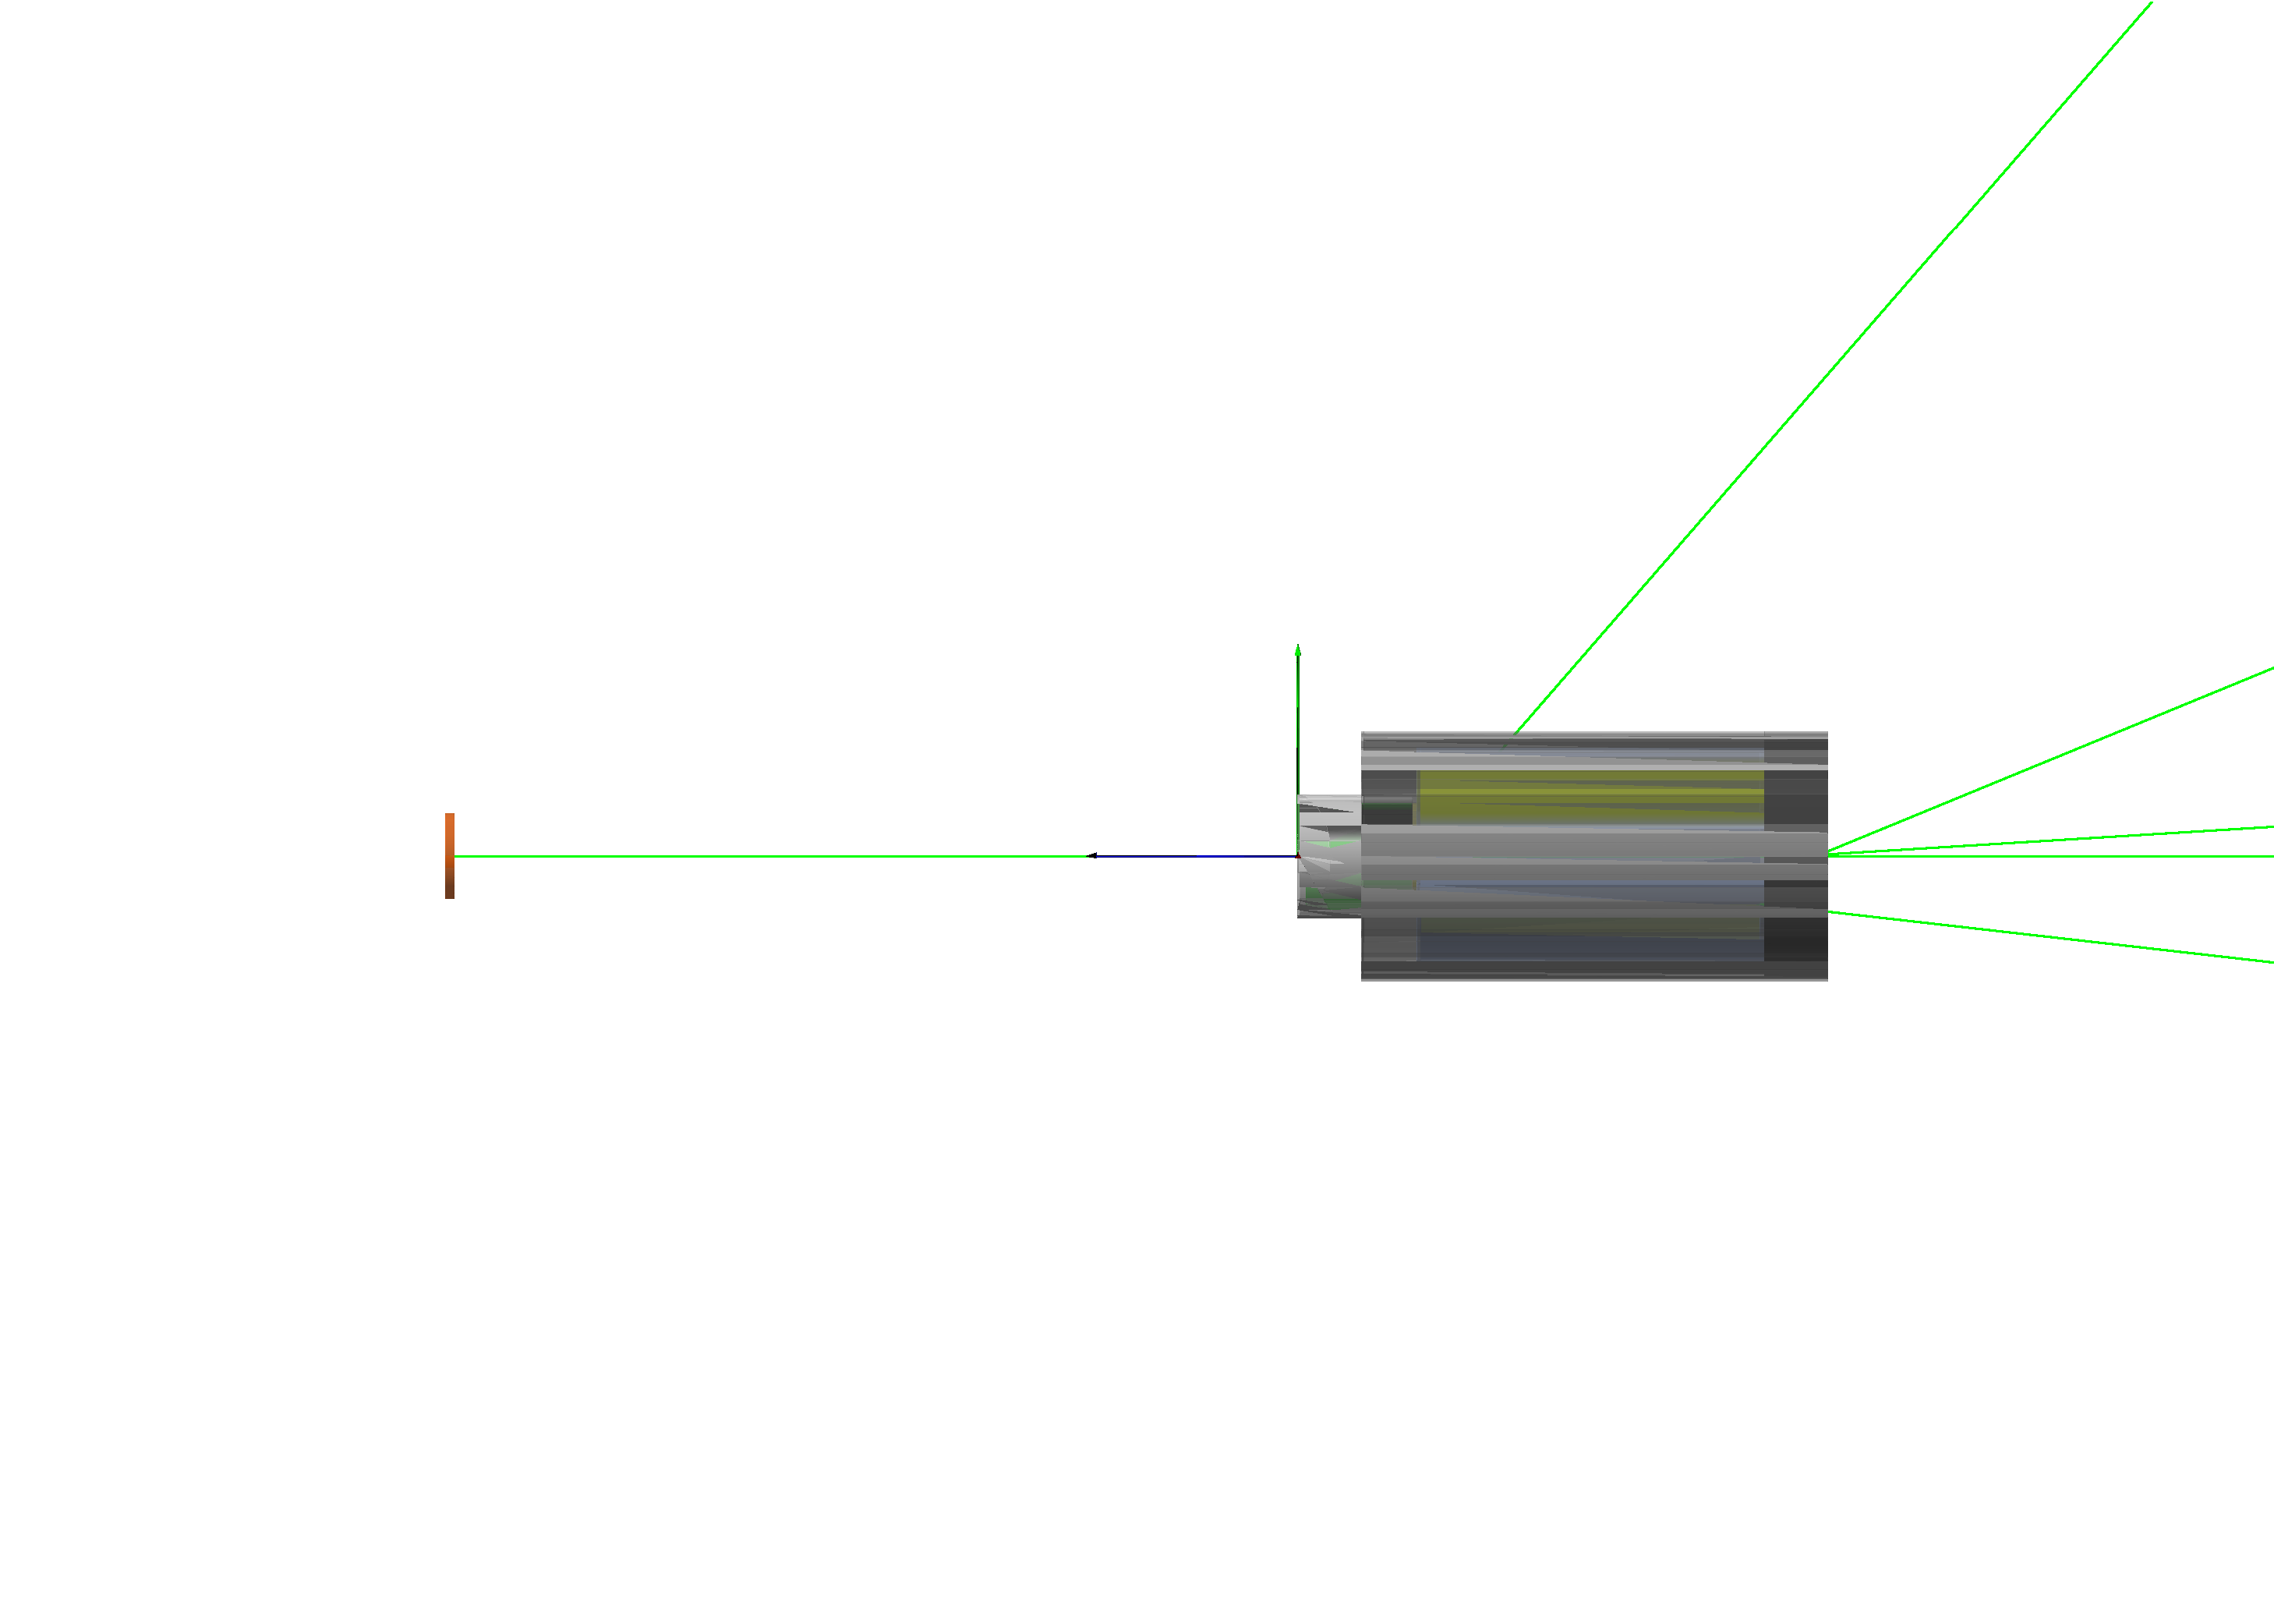
\includegraphics[width=\linewidth]{fig_vis_side.pdf}\\[2pt]
  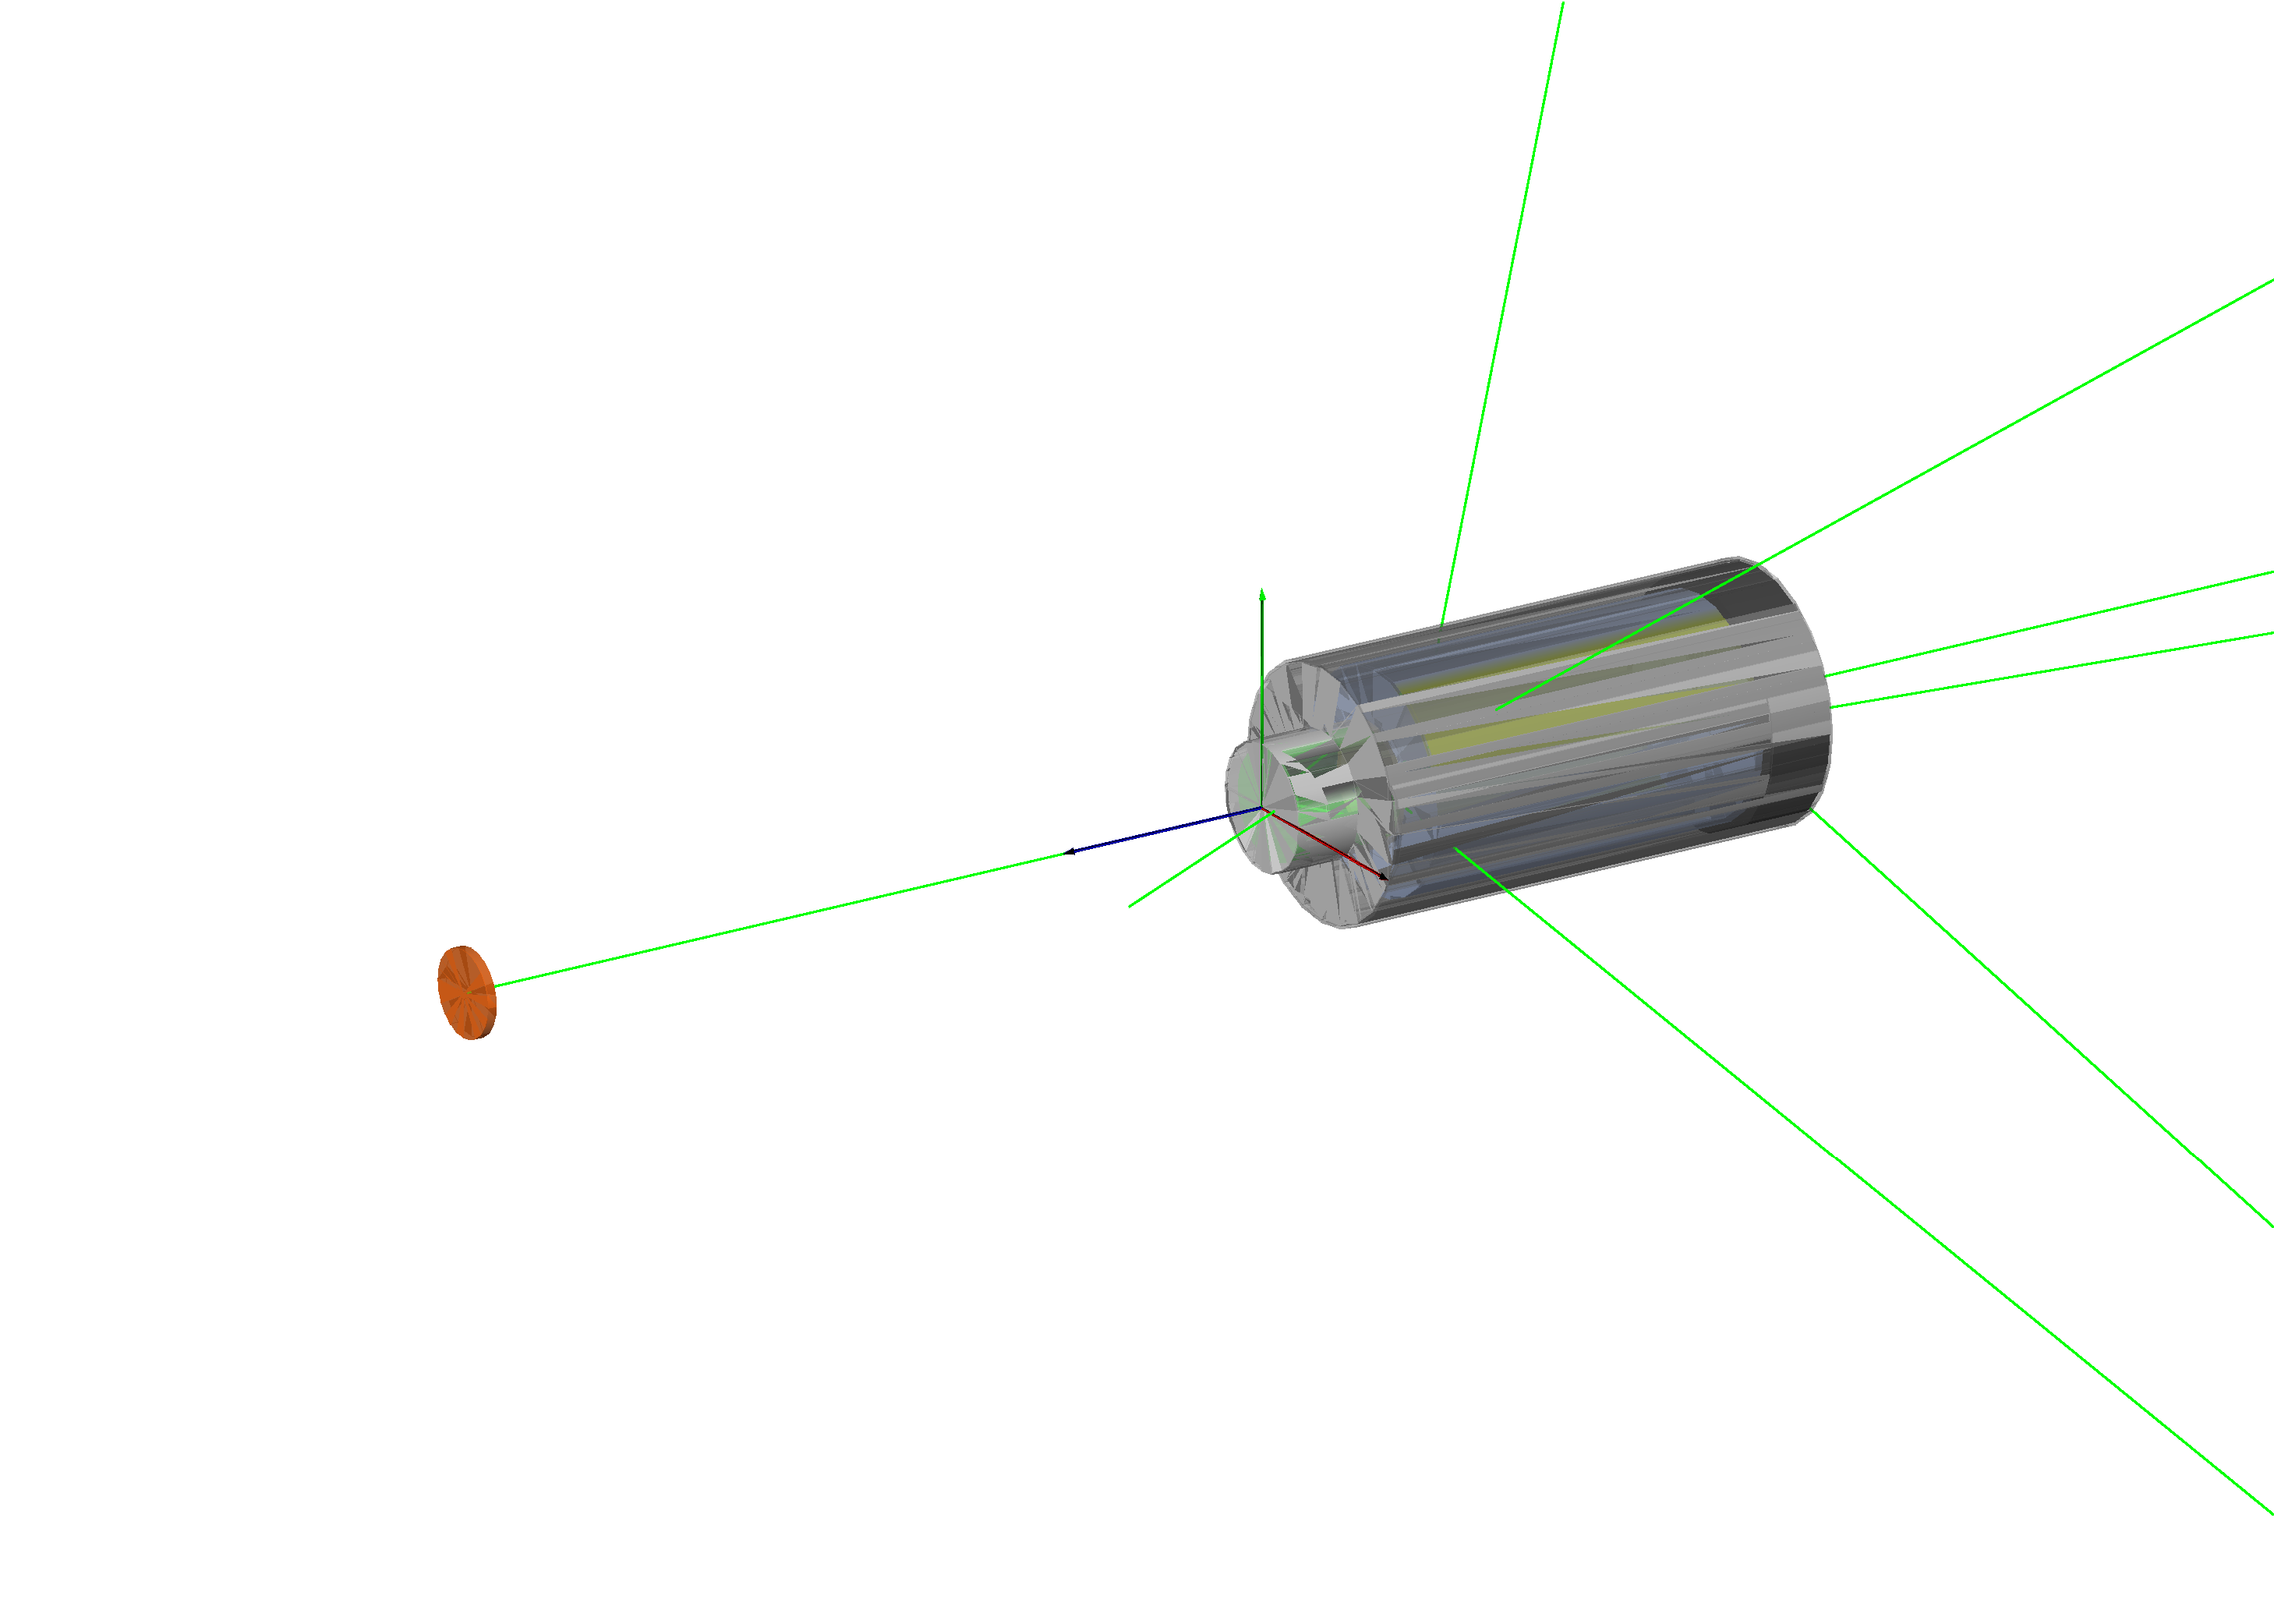
\includegraphics[width=0.82\linewidth]{fig_vis_oblique.pdf}
  \caption{Geant4/OpenGL event displays for ten \SI{661.64}{keV} gammas from
  the source puck at \SI{200}{mm}. Top: side view along the detector axis;
  the source puck appears edge-on at the left and the detector is at the
  right. Bottom: oblique view showing the puck, the detector body, the crystal,
  and the tracks. The source is focused toward the detector only for these
  renders; the production source is isotropic.}
  \label{fig:vis}
\end{figure}

\section{Simulation method}

\subsection{Production matrix and physics}

The production matrix is three distances times three energies, with
\num{1e7} incident gammas per point. The runs use the \texttt{G4DCSmonitor}
binary built from this repository, the \texttt{GPS} source mode, and the
physics list in \texttt{PhysicsList.cc}: \texttt{G4EmStandardPhysics\_option4}
for electromagnetic transport, with hadronic HP, thermal-neutron, ion, and
gamma-nuclear components included for the full simulation. The gamma
efficiency is controlled by the electromagnetic physics and the geometry; the
hadronic components do not contribute at these energies.

The source is a point at the puck centre with an isotropic angular
distribution. The detector geometry includes the crystal, the detector body,
and the magnesium shield. The production macro writes the \texttt{hits} tree
and the \texttt{meta} tree. The \texttt{hits} tree stores one row per pulse;
the analysis sums all rows with the same event number to recover the total
energy deposited in the crystal per event. The analysis uses detector
identifier \num{0} for the CLYC crystal and ignores zero-weight rows.

\begin{table}[H]
  \centering
  \caption{Simulation production matrix and full-energy peak counts. Each point
  uses \num{1e7} incident gammas. $N_{\mathrm{peak}}$ counts events whose total
  energy deposition lies within $\pm\SI{2}{\percent}$ of the incident energy.
  The last column is the relative statistical uncertainty
  $\sqrt{N_{\mathrm{peak}}}/N_{\mathrm{peak}}$, expressed as a percentage.}
  \label{tab:sim}
  \small
  \begin{tabular}{@{}rrrrrr@{}}
    \toprule
    $d$ [mm] & $E$ [keV] & $N_{\mathrm{inc}}$ & $N_{\mathrm{peak}}$ &
    $\epsilon_{\mathrm{sim}}$ [\%] & rel. stat [\%] \\
    \midrule
    200 & 661.64  & \num{1e7} & 843 & \num{0.00843(29)} & 3.4 \\
    200 & 1173.23 & \num{1e7} & 384 & \num{0.00384(20)} & 5.1 \\
    200 & 1332.51 & \num{1e7} & 326 & \num{0.00326(18)} & 5.5 \\
    300 & 661.64  & \num{1e7} & 385 & \num{0.00385(20)} & 5.1 \\
    300 & 1173.23 & \num{1e7} & 166 & \num{0.00166(13)} & 7.8 \\
    300 & 1332.51 & \num{1e7} & 148 & \num{0.00148(12)} & 8.2 \\
    400 & 661.64  & \num{1e7} & 205 & \num{0.00205(14)} & 7.0 \\
    400 & 1173.23 & \num{1e7} & 106 & \num{0.00106(10)} & 9.7 \\
    400 & 1332.51 & \num{1e7} & 71  & \num{0.00071(8)}  & 11.9 \\
    \bottomrule
  \end{tabular}
\end{table}

\subsection{Efficiency definitions and analysis}

The simulated full-energy peak efficiency is
\begin{equation}
  \epsilon_{\mathrm{sim}}
  = \frac{N_{\mathrm{peak}}}{N_{\mathrm{inc}}}\times 100,
  \label{eq:eff-sim}
\end{equation}
where $N_{\mathrm{inc}}=\num{1e7}$ and $N_{\mathrm{peak}}$ is the number of
events with
\begin{equation}
  (1-0.02)E \le E_{\mathrm{dep}} \le (1+0.02)E.
  \label{eq:window}
\end{equation}
The $\pm\SI{2}{\percent}$ window captures the full-energy peak and excludes the
single-escape peak at $E-\SI{511}{keV}$ and the double-escape peak at
$E-\SI{1022}{keV}$. The simulation has no detector resolution, so the
full-energy peak is a delta function; the window is wide enough to contain it
and narrow enough to exclude the escape peaks. The statistical uncertainty is
\begin{equation}
  \sigma_{\mathrm{sim}}
  = \frac{\sqrt{N_{\mathrm{peak}}}}{N_{\mathrm{inc}}}\times 100.
  \label{eq:eff-sim-error}
\end{equation}
The measured efficiency is given by Eq.~\eqref{eq:eff-exp}; its statistical
uncertainty is dominated by the net peak area,
\begin{equation}
  \sigma_{\mathrm{meas}}
  = \frac{\epsilon_{\mathrm{meas}}}{\sqrt{N_{\mathrm{peak}}}}.
  \label{eq:eff-meas-error}
\end{equation}
The simulation-to-measurement ratio is
\begin{equation}
  R = \frac{\epsilon_{\mathrm{sim}}}{\epsilon_{\mathrm{meas}}},
  \qquad
  \sigma_R = R\sqrt{
    \left(\frac{\sigma_{\mathrm{sim}}}{\epsilon_{\mathrm{sim}}}\right)^2
    +
    \left(\frac{\sigma_{\mathrm{meas}}}{\epsilon_{\mathrm{meas}}}\right)^2
  }.
  \label{eq:ratio}
\end{equation}
The pull is
\begin{equation}
  \mathrm{pull}
  = \frac{\epsilon_{\mathrm{sim}}-\epsilon_{\mathrm{meas}}}
  {\sqrt{\sigma_{\mathrm{sim}}^2+\sigma_{\mathrm{meas}}^2}}.
  \label{eq:pull}
\end{equation}

\section{Results}

\subsection{Efficiency versus distance}

Figure~\ref{fig:eff} shows the simulated and measured full-energy peak
efficiencies as functions of distance. The simulation points are filled
markers connected by lines; the measurement points are open markers. The
vertical axis is logarithmic because the efficiency falls by an order of
magnitude between \SI{200}{mm} and \SI{400}{mm}. The \SI{661.64}{keV} curves
overlap within the marker size at \SI{200}{mm} and separate by up to
\SI{9}{\percent} at the larger distances. The \SI{1173.23}{keV} and
\SI{1332.51}{keV} simulation curves lie above the measurement at every
distance, with the largest separation at \SI{200}{mm}.

\begin{figure}[H]
  \centering
  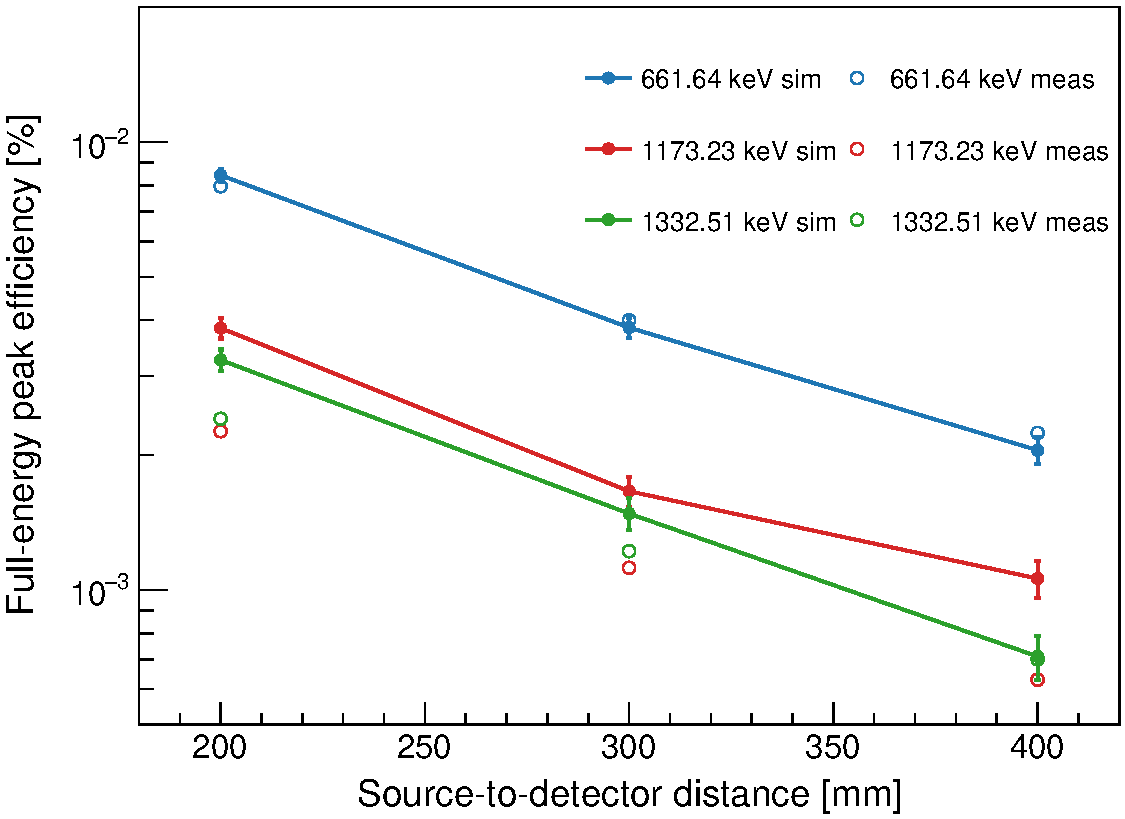
\includegraphics[width=\linewidth]{fig_eff_vs_distance.pdf}
  \caption{Full-energy peak efficiency versus source-to-detector distance for
  the three gamma lines. Filled markers and solid lines are the simulation;
  open markers are the measurement. The vertical axis is logarithmic. The
  simulation uses \num{1e7} incident gammas per point; the error bars are the
  statistical uncertainties of Eqs.~\eqref{eq:eff-sim-error}
  and~\eqref{eq:eff-meas-error}.}
  \label{fig:eff}
\end{figure}

\subsection{Ratio and energy dependence}

Figure~\ref{fig:ratio} shows $R=\epsilon_{\mathrm{sim}}/
\epsilon_{\mathrm{meas}}$. The shaded band is $\pm\SI{10}{\percent}$ around
$R=1$, and the dashed line is $R=1$. The \SI{661.64}{keV} points lie inside
the band at all three distances. The \SI{1173.23}{keV} points lie above the
band at all three distances; the ratios are \num{1.699}, \num{1.482}, and
\num{1.683}. The \SI{1332.51}{keV} points are \num{1.353} at \SI{200}{mm},
\num{1.213} at \SI{300}{mm}, and \num{1.014} at \SI{400}{mm}; the first two
are above the band, while the last is inside it.

\begin{figure}[H]
  \centering
  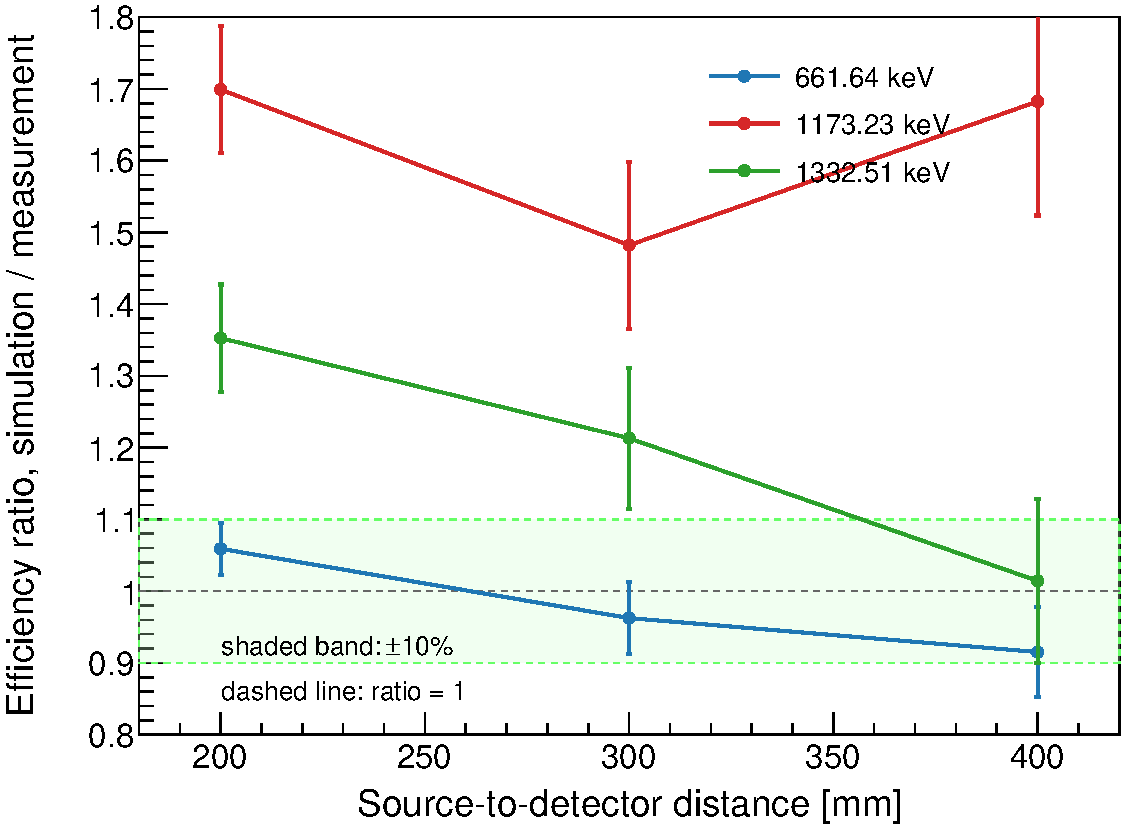
\includegraphics[width=0.92\linewidth]{fig_eff_ratio.pdf}
  \caption{Simulation-to-measurement efficiency ratio versus distance. The
  shaded band is $\pm\SI{10}{\percent}$ around $R=1$; the dashed line is
  $R=1$. The error bars follow Eq.~\eqref{eq:ratio}. The \SI{661.64}{keV}
  points are consistent with unity; the \SI{1173.23}{keV} and
  \SI{1332.51}{keV} points are high, except for the \SI{400}{mm}
  \SI{1332.51}{keV} point.}
  \label{fig:ratio}
\end{figure}

Table~\ref{tab:comparison} collects the numerical comparison. The pull column
uses Eq.~\eqref{eq:pull}. The \SI{661.64}{keV} pulls are \num{1.6},
\num{-0.8}, and \num{-1.4}; none is significant at the $2\sigma$ level.
The \SI{1173.23}{keV} pulls are \num{7.9}, \num{4.2}, and \num{4.3}; all are
significant. The \SI{1332.51}{keV} pulls are \num{4.7}, \num{2.2}, and
\num{0.1}; the \SI{200}{mm} and \SI{300}{mm} points are significant, while the
\SI{400}{mm} point is not.

\begin{table}[H]
  \centering
  \caption{Comparison of simulated and measured full-energy peak efficiencies.
  The measured values are the corrected CSV values from
  Eq.~\eqref{eq:csv-correction}. The ratio and pull follow
  Eqs.~\eqref{eq:ratio} and~\eqref{eq:pull}. The simulation uncertainty is
  statistical only; the measured uncertainty is the Poisson error on the net
  peak area.}
  \label{tab:comparison}
  \small
  \begin{tabular}{@{}rrrrrr@{}}
    \toprule
    $d$ [mm] & $E$ [keV] & $\epsilon_{\mathrm{sim}}$ [\%] &
    $\epsilon_{\mathrm{meas}}$ [\%] & $R$ & pull \\
    \midrule
    200 & 661.64  & \num{0.00843(29)} & 0.00796 & 1.059 & 1.6 \\
    200 & 1173.23 & \num{0.00384(20)} & 0.00226 & 1.699 & 7.9 \\
    200 & 1332.51 & \num{0.00326(18)} & 0.00241 & 1.353 & 4.7 \\
    300 & 661.64  & \num{0.00385(20)} & 0.00400 & 0.963 & -0.8 \\
    300 & 1173.23 & \num{0.00166(13)} & 0.00112 & 1.482 & 4.2 \\
    300 & 1332.51 & \num{0.00148(12)} & 0.00122 & 1.213 & 2.2 \\
    400 & 661.64  & \num{0.00205(14)} & 0.00224 & 0.915 & -1.4 \\
    400 & 1173.23 & \num{0.00106(10)} & 0.00063 & 1.683 & 4.3 \\
    400 & 1332.51 & \num{0.00071(8)}  & 0.00070 & 1.014 & 0.1 \\
    \bottomrule
  \end{tabular}
\end{table}

The measured \SI{1173.23}{keV}/\SI{1332.51}{keV} ratio is \num{0.94} at
\SI{200}{mm}, \num{0.92} at \SI{300}{mm}, and \num{0.90} at \SI{400}{mm}. The
CSV reference column gives \num{1.21}; the simulation gives \num{1.18},
\num{1.12}, and \num{1.49}. The measured ratio is therefore inverted: the
\SI{1332.51}{keV} peak is larger than the \SI{1173.23}{keV} peak at every
distance, while the reference and the simulation both put the
\SI{1173.23}{keV} peak above the \SI{1332.51}{keV} peak. The \SI{400}{mm} simulation ratio of \num{1.49} is higher than the
reference ratio because the \SI{400}{mm} \SI{1332.51}{keV} point has only
$N_{\mathrm{peak}}=71$ and an \SI{11.9}{\percent} statistical uncertainty; the
ratio is correspondingly imprecise.

\subsection{Spectra at \SI{200}{mm}}

Figure~\ref{fig:spectra} shows the simulated total-energy-deposition spectra
at \SI{200}{mm} for the three energies. The histograms are normalised to
\num{1e7} incident gammas and to the bin width in keV, so the vertical axis is
events per \num{1e7} incident gammas per keV. The dashed vertical lines mark
the $\pm\SI{2}{\percent}$ window and the central line marks the incident
energy. The \SI{661.64}{keV} spectrum has a clear full-energy peak at
\SI{661.64}{keV}. The \SI{1173.23}{keV} and \SI{1332.51}{keV} spectra have
smaller full-energy peaks on a Compton continuum; the peaks are still visible
above the continuum, and the $\pm\SI{2}{\percent}$ window contains them.

\begin{figure}[H]
  \centering
  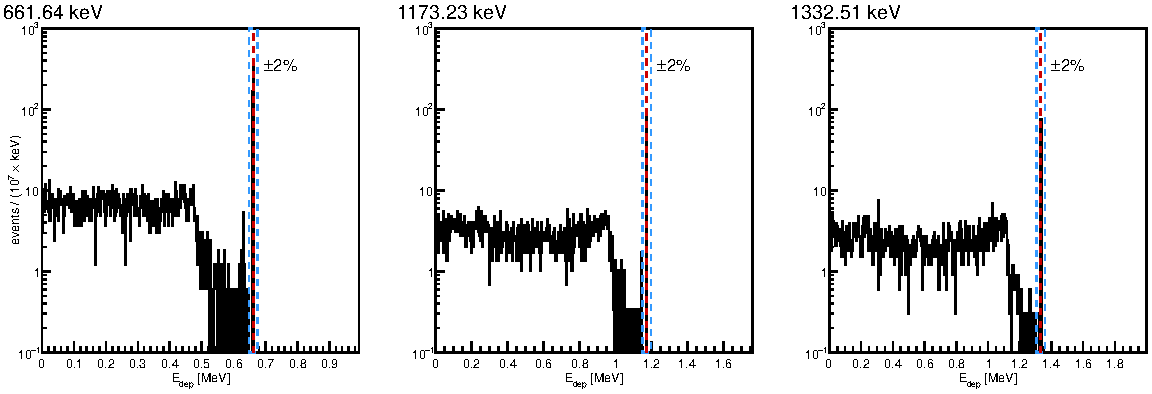
\includegraphics[width=\linewidth]{fig_spectra_200mm.pdf}
  \caption{Simulated total energy deposition spectra at \SI{200}{mm} for
  \SI{661.64}{keV}, \SI{1173.23}{keV}, and \SI{1332.51}{keV}. The histograms
  are normalised to \num{1e7} incident gammas per keV. The dashed vertical
  lines mark the $\pm\SI{2}{\percent}$ window; the central line marks the
  incident energy. The full-energy peaks are the sharp structures at the
  incident energies; the lower continuum is Compton scattering in the crystal
  and the surrounding material.}
  \label{fig:spectra}
\end{figure}

\subsection{No-puck control}

The no-puck control uses the same geometry and source position as the
\SI{200}{mm} \SI{661.64}{keV} point, but omits the epoxy puck. The control
gives $\epsilon_{\mathrm{sim}}=\num{0.00876(30)}\,\%$, compared with
\num{0.00843(29)}\,\% with the puck. The ratio is \num{1.100}. The fractional
change is
\begin{equation}
  \frac{\epsilon_{\mathrm{with\ puck}}-\epsilon_{\mathrm{no\ puck}}}
  {\epsilon_{\mathrm{no\ puck}}}
  = -\SI{3.8 \pm 4.8}{\percent}.
  \label{eq:nopuck}
\end{equation}
The puck therefore changes the \SI{661.64}{keV} efficiency by less than
\SI{10}{\percent} at the $1\sigma$ level. The puck attenuation at
\SI{1173.23}{keV} and \SI{1332.51}{keV} is smaller than at \SI{661.64}{keV},
so the puck cannot explain the \num{1.5}--\num{1.7} factor at
\SI{1173.23}{keV} or the \num{1.2}--\num{1.35} factor at
\SI{1332.51}{keV}. The control supports the conclusion that the discrepancy is
in the detector response or the source model, not in the source encapsulation.

\section{Discussion}

\subsection{What the \SI{661.64}{keV} agreement shows}

The \SI{661.64}{keV} ratios are \num{1.059}, \num{0.963}, and \num{0.915}.
The corresponding pulls are \num{1.6}, \num{-0.8}, and \num{-1.4}. The
simulation and measurement therefore agree within the combined statistical
uncertainties at all three distances. This agreement tests several ingredients
at once: the crystal diameter and length, the \SI{2}{mm} crystal recess, the
source-to-detector distance, the $\pm\SI{2}{\percent}$ analysis window, and
the conversion from the CSV efficiency to the corrected measured efficiency.
A \SI{10}{\percent} error in the crystal radius would change the efficiency by
about \SI{20}{\percent}; a \SI{10}{\percent} error in the source distance would
change it by about \SI{20}{\percent} at \SI{200}{mm} and less at
\SI{400}{mm}. Both would be larger than the observed \SI{661.64}{keV}
differences.

The agreement does not validate the absolute efficiency at the
\SI{1}{\percent} level. The simulation/measurement ratio is \num{1.059} at
\SI{200}{mm}, \num{0.963} at \SI{300}{mm}, and \num{0.915} at \SI{400}{mm}.
The pattern is not monotonic; it is consistent with the
\SI{3}{}--\SI{7}{\percent} statistical errors of the simulation and the
\SI{0.5}{\percent} statistical errors of the measurement, plus the systematic
uncertainties that are not yet quantified. The \SI{661.64}{keV} result is a \SI{10}{\percent}-level
validation, not a precision calibration.

\subsection{Why \SI{1173.23}{keV} and \SI{1332.51}{keV} disagree}

The \SI{1173.23}{keV} simulation is high by \SI{48}{}--\SI{70}{\percent}; the
\SI{1332.51}{keV} simulation is high by \SI{1}{}--\SI{35}{\percent}. The
discrepancy is energy dependent: it is small at \SI{661.64}{keV}, large at
\SI{1173.23}{keV}, and intermediate at \SI{1332.51}{keV}. A geometric error
would scale all three energies similarly, because the geometric acceptance is
independent of energy. The \SI{661.64}{keV} agreement therefore argues against
a geometry error as the primary cause.

The most plausible source-model difference is that the simulation generates
one monoenergetic gamma per event, while \ce{^{60}Co} emits
\SI{1173.23}{keV} and \SI{1332.51}{keV} gammas in cascade. In the measurement,
the two gammas can deposit energy in the crystal in the same event. True
coincidence summing can add counts to a full-energy peak (summing in) or
remove counts from it (summing out), depending on the source--detector
geometry and the surrounding material. The simulation does not include the
cascade, so it cannot reproduce either effect. The measured
\SI{1173.23}{keV}/\SI{1332.51}{keV} ratio is inverted relative to the
reference and the simulation; cascade summing is a plausible explanation for
an energy-dependent change of this sign and size. The present data do not
prove this explanation, because the CSV contains net peak areas rather than
spectra and the simulation has no coincidence model. A \ce{^{60}Co} cascade
source in Geant4, with both gammas emitted in the same event, is the direct
test.

A second source-model difference is the detector response. The simulation
records total energy deposition and applies a $\pm\SI{2}{\percent}$ window. The
measurement fits a full-energy peak with a finite resolution and a background.
If the \SI{1173.23}{keV} and \SI{1332.51}{keV} peaks sit on a larger Compton
background than the \SI{661.64}{keV} peak, the peak-fit area can be biased by
the background model. The measured spectra are not in the CSV, so this effect
cannot be separated from cascade summing with the present data. A consistent
peak-fit procedure applied to the measured spectra, and a simulation with
detector resolution and a realistic background, are needed.

A third possibility is an error in the source activity or the emission
probability for \ce{^{60}Co}. The measured \SI{1173.23}{keV} and
\SI{1332.51}{keV} efficiencies use the same current activity
(\SI{11.31e6}{Bq}) and nearly the same emission probabilities
(\SI{99.97}{\percent} and \SI{99.99}{\percent}). A common activity error would
shift both efficiencies by the same factor and would not invert their ratio.
An error in the ratio of the two emission probabilities would have to be about
\SI{30}{\percent} to explain the measured \num{0.90} ratio, which is much
larger than the quoted values. The activity explanation is therefore less
likely than the cascade or peak-fit explanations, but it is not excluded
without an independent activity measurement.

The \SI{200}{mm} measured points are lower than the \SI{300}{mm} and
\SI{400}{mm} trends. The \SI{661.64}{keV} \SI{200}{mm} point is
\SI{5.6}{\percent} below the simulation, while the \SI{1173.23}{keV} and
\SI{1332.51}{keV} \SI{200}{mm} points are \SI{41}{\percent} and
\SI{26}{\percent} below. The close geometry increases the solid angle and the
probability of cascade summing, so the larger discrepancy at \SI{200}{mm} is
qualitatively consistent with the cascade hypothesis. A source-distance error
of a few millimetres would change the geometric acceptance by a few percent,
not by \SI{40}{\percent}; the \SI{661.64}{keV} point at the same distance is
consistent with the simulation, so a common distance error is unlikely.

\subsection{Intrinsic efficiency}

Dividing the full-energy peak efficiency by the geometric acceptance of
Eq.~\eqref{eq:omega} removes the leading distance dependence. The
\SI{661.64}{keV} intrinsic efficiency is \num{0.083}--\num{0.094} for both
the simulation and the measurement, with no significant distance trend. The
\SI{1173.23}{keV} measured intrinsic efficiency is \num{0.024}--\num{0.026},
compared with \num{0.039}--\num{0.044} in the simulation. The
\SI{1332.51}{keV} measured intrinsic efficiency is \num{0.025}--\num{0.029},
compared with \num{0.029}--\num{0.035} in the simulation. The
\SI{661.64}{keV} agreement and the \SI{1173.23}{keV} disagreement are
therefore properties of the detector response, not of the distance scaling.
This is the strongest argument that the geometric acceptance and the source
placement are not the primary problem.

\subsection{Limitations}

The comparison has several limitations. The simulation statistical
uncertainties are \SI{3}{}--\SI{12}{\percent}; the \SI{400}{mm}
\SI{1332.51}{keV} point has only \num{71} peak events. The measured
statistical uncertainties are \SI{0.25}{}--\SI{0.5}{\percent}, but the
systematic uncertainties of the activity, the distance, the detector
geometry, and the peak fitting are not included. The simulation has no
detector resolution, no scintillation light, no light-collection efficiency,
and no electronics threshold. The measured efficiency is a full-energy peak
efficiency from a fit; the simulated efficiency is a total-energy-deposition
window. The two definitions are close but not identical. The CSV contains net
peak areas rather than spectra, so the peak-fit method cannot be checked. The
\ce{^{60}Co} cascade is not simulated. The reference column of the CSV is not
the measured efficiency and is not used as a denominator; it is used only for
the energy-dependence comparison. These limitations do not affect the
\SI{661.64}{keV} conclusion, but they limit the interpretation of the
\SI{1173.23}{keV} and \SI{1332.51}{keV} discrepancies.

\section{Conclusion and next steps}

The CLYC simulation reproduces the measured \SI{661.64}{keV} full-energy peak
efficiency within \SI{9}{\percent} at \SI{200}{mm},
\SI{300}{mm}, and \SI{400}{mm}. The agreement validates the detector geometry,
the \SI{2}{mm} crystal recess, the source distance, the $\pm\SI{2}{\percent}$
analysis window, and the correction of the CSV efficiency by a factor of
\num{1000}. The simulation overestimates the \SI{1173.23}{keV} efficiency by
\SI{48}{}--\SI{70}{\percent} and the \SI{1332.51}{keV} efficiency by
\SI{1}{}--\SI{35}{\percent}; the \SI{1173.23}{keV} discrepancy is significant
at $4$--$8\sigma$. The measured
\SI{1173.23}{keV}/\SI{1332.51}{keV} ratio is \num{0.90}{}--\num{0.94}, while
the reference and the simulation give \num{1.21} and \num{1.12}{}--%
\num{1.49}. The no-puck control changes the \SI{661.64}{keV} efficiency by
\SI{3.8 \pm 4.8}{\percent}, so the epoxy puck is not the cause.

The next steps are:
\begin{enumerate}
  \item Simulate \ce{^{60}Co} as a cascade source, with both the
        \SI{1173.23}{keV} and \SI{1332.51}{keV} gammas emitted in the same
        event, and compare the coincidence-summed full-energy peaks with the
        measurement.
  \item Add a detector response model with energy resolution, a light-collection
        efficiency, and an electronics threshold, and fit the simulated
        spectra with the same peak model used for the measured spectra.
  \item Obtain the measured spectra and repeat the peak fit with a consistent
        background model; check whether the \SI{1173.23}{keV} and
        \SI{1332.51}{keV} net peak areas change.
  \item Measure the source activity and the source-to-detector distance
        independently, and propagate their uncertainties into the efficiency.
  \item Extend the matrix to more distances and energies, and add a full
        systematic uncertainty budget before using the simulation for a
        calibration.
\end{enumerate}

\appendix

\section{Reproducing the efficiency scan}

The production scan is driven by
\texttt{scripts/run\_clyc\_eff\_gamma.sh}. The default production mode uses
\num{1e7} events per point and the nine-point matrix:
\begin{verbatim}
cmake --build build -j
scripts/run_clyc_eff_gamma.sh --production
\end{verbatim}
The driver writes the macros, logs, and ROOT files to
\texttt{build/validation/clyc\_eff/}. The no-puck control is
\begin{verbatim}
scripts/run_clyc_eff_gamma.sh --nev 10000000 --nopuck \
  --distances 200 --energies 661.64
\end{verbatim}
The efficiency analysis is
\texttt{scripts/analyze\_clyc\_eff.C}; one point is analysed with
\begin{verbatim}
root -l -b -q \
  'scripts/analyze_clyc_eff.C("build/validation/clyc_eff/\
clyc_eff_200mm_661p64keV.root",661.64,10000000,0.00796)'
\end{verbatim}
and the same call is repeated for the other eight points with the
corresponding energy and corrected CSV efficiency. The report figures are
generated by
\begin{verbatim}
root -l -b -q report/eff_clyc/scripts/make_eff_figs.C
\end{verbatim}
The event displays are generated by
\begin{verbatim}
bash report/eff_clyc/scripts/make_vis_figs.sh
\end{verbatim}
The display macros use ten events and a focused source for visibility; they do
not change the production macros or the efficiency results.

\section{Data and code locations}

\begin{itemize}
  \item Measurement: \texttt{/home/turko46/data/CLYC\_validation/effDist\_clyc1.csv}.
  \item Production outputs: \texttt{build/validation/clyc\_eff/}.
  \item Efficiency analysis: \texttt{scripts/analyze\_clyc\_eff.C}.
  \item Production driver: \texttt{scripts/run\_clyc\_eff\_gamma.sh}.
  \item Production templates: \path{macros/validation/clyc_eff_gamma_template.mac}
        and \path{macros/validation/clyc_eff_gamma_nopuck_template.mac}.
  \item Detector geometry: \texttt{src/GeometryCLYC.cc} and
        \texttt{src/DetectorConstruction.cc}.
  \item Source placement: \texttt{src/PrimaryGeneratorAction.cc}.
  \item Physics list: \texttt{src/PhysicsList.cc}.
  \item Report figures: \texttt{report/eff\_clyc/figures/}.
  \item Figure scripts: \texttt{report/eff\_clyc/scripts/}.
  \item Event-display macros: \texttt{report/eff\_clyc/vis/}.
\end{itemize}

\end{document}
